
%FIXME: put results of the cluster and oprganize residuals part
By this point, the report brought up all the tools we need for an application of the InexactGMRES algorithm, from the algorithm itself to the way we generate the coefficient matrices used in the linear equations.

Before we use the main algorithm directly in a more complex problem, we start out with simpler geometries, to first validate the speedup obtained in a simple matrix-vector product with different tolerances. We then apply the Inexact GMRES in the problem of a cavity scattering, known for taking a larger number of iterations in the standard GMRES.

\section{Validation of the inexact matrix-vector product}

For the first test, we use Laplace's equation (first line in \ref{eq:pde_model}, and that we repeat here for context) to generate our first coefficient matrix. The second matrix-vector product example will use Helmholtz's equation, the second line in the following equation:

\begin{align}\label{eq:edp_examples}
    \begin{split}
        \Delta u &= 0\\
        \Delta u + k^{2}u &=0
    \end{split}
\end{align}

With $k$ the wave number associated with the solution.

%FIXME:maybe more details about the quadrature, etc
%FIXME: Put a figure of the unite circle?
As for the geometry, we choose a unit circle around the origin as the boundary, using the Inti library \cite{git-inti} to go through all steps in \autoref{chap:bemethod}.


The first coefficient matrix $A_{L}$ is made from the fundamental solution of Laplace's equation, the first line in \autoref{eq:edp_examples}, after transforming it into an integral equation, through the single layer potential mentioned in \autoref{eq:singlelayer_pot}.

With $\gamma(x,y)$ the fundamental solution of Laplace's equation:

\begin{equation}
    \gamma (x,y) = \frac{-1}{2\pi} \log |x-y| \hspace{0.2in} (x,y \in \mathbb{R}^{2})
\end{equation}

The coefficient matrix $A_{H}$ for the second example is generated from Helmholtz's equation, second line in \autoref{eq:edp_examples}, using the single and double layer potentials in \autoref{eq:singlelayer_pot} and \autoref{eq:doublelayer_pot}. The fundamental solution of the differential equation is:

\begin{equation}
    \gamma(x,y) = \frac{i}{4} H_{0}^{(1)}(k|x-y|)
\end{equation}

The Hankel function of the first kind.

%FIXME: put inf tolerance results here
Before going into each one of the results, we talk a little about both extremes of the performance evaluation in the matrix-vector problem. How to give an upper bound to the acceleration we expect?

If making the matrix-vector product's tolerance as 0 implies the use of the “original”   matrix(hierarchical matrices are already an approximation). Then, we would expect 0$\%$ speedup and $t_{exact}$, the execution time for the exact product, to be equal to $t_{inexact}$, the execution time for the inexact version.

A good way to infer an upper bound for the inexact products would be using only rank 1 blocks for the admissible ones and measuring its execution time. To do that, we change the product tolerance to a very large value, \textit{inf} from Julia, and the product will be realized with only rank-1 blocks, since it's programmed to get the first approximation lower than its given tolerance.

Of course, such thing would not happen in a practical situation, but it gives an upper bound for the speedup we should expect, the maximum value $\frac{t_{exact}}{t_{inexact}}$ could attain.

To assemble both hierarchical matrices, $A_{L}$ and $A_{H}$, we use an overall tolerance $\epsilon$ of $10^{-8}$. The results for the speed-ups and the relative residual for each product tolerance, $\nu$, are in \autoref{fig:product_results}.

\begin{figure}[h!]
    \centering
    \begin{subfigure}[b]{0.45\linewidth}
        \includesvg[width=\linewidth]{images/speedup_products.svg}
        \caption{Speed-ups for the inexact product of a hierarchical matrix and a vector.}
    \end{subfigure}
    \begin{subfigure}[b]{0.45\linewidth}
        \includesvg[width=\linewidth]{images/residuals_products.svg}
        \caption{Relative residuals for inexact product of a hierarchical matrix and a vector.}
    \end{subfigure}
    \caption{Results for the initial example of a inexact product. The coefficient matrices have dimensions 62835 $\times$ 62835 and were assembled with an overall tolerance $\epsilon = 10^{-8}$.}
    \label{fig:product_results}
\end{figure}

We leave the identity curve in the plot on the right due to compare each inexact product's residual with the minimum accuracy that should be satisfied by its resulting vector. And since the matrix-product is accelerated, we should expect some speedup in the algorithm as well.

For a second evaluation of the inexact product, we change our setup. Fixing the product tolerance $\nu=10^{-6}$, now the dimensions of $A_{L}$ and $A_{H}$ are variable, with both still being assembled with tolerance $10^{-8}$. The observed speed-ups are in \autoref{fig:product_fixtol_results}.

\begin{figure}[h!]
    \centering
    \begin{subfigure}[b]{0.45\linewidth}
        \includesvg[width=\linewidth]{images/speedup_productsfixtol.svg}
        \caption{Speed-ups for the inexact product of a hierarchical matrix and a vector.}
    \end{subfigure}
    \begin{subfigure}[b]{0.45\linewidth}
        \includesvg[width=\linewidth]{images/residuals_productsfixtol.svg}
        \caption{Relative residuals for inexact product of a hierarchical matrix and a vector.}
    \end{subfigure}
    \caption{Results for the initial example of a inexact product. The products are executed with tolerance $\nu=10^{-6}$ and the hierarchical matrices assembled with an overall tolerance $\epsilon = 10^{-8}$.}
    \label{fig:product_fixtol_results}
\end{figure}

%FIXME: talk a little about what these curves mean 

It should be noted that the acceleration is highly dependent on the compression of the coefficient matrix. Matrices with low maximum rank of each block would not receive a big boost, since the number of columns used for each sub-block might not vary much with each different tolerance.



\section{Cavity scattering}

\subsection{Tolerance heuristic}

We mentioned the inexact product's tolerance, $\nu$, multiple times throughout this study, but haven't really disclosed \textbf{how} to obtain it. For the simple example of the matrix-vector product of before, we could simply define it as we please, but the situation changes for the Inexact GMRES. For the latter, everything needs to be made as to give a converging solution, specially to respect all bound found in the inexact session of \autoref{chap:gmres}.

As told in \autoref{chap:hmatrices}, we adjust the inexact matrix-vector product with the number of columns used by each one of the subblocks during the operation.

We use a heuristic to obtain, at each iteration $k$, a product tolerance $\nu_{k}$ as to keep $||E_{k}||$ lower than the bounds in \autoref{eq:bound_E} or \autoref{eq:boundE_final}. Then $\nu_{k}$ is later converted to an integer, the number of columns used by each admissible block, through algorithm \ref{alg:inexact_product}.

The following formula, used in \cite{wang2016inexactkryloviterationsrelaxation}, is equivalent to setting $\ell_{k}$ in \autoref{eq:boundE_final} as 1.

\begin{equation}\label{eq:gen_heuristics}
    \nu_{k} = \min \left(\frac{\epsilon}{\min(\tilde{r}_{k-1},1)},1 \right)
\end{equation}

Where $\tilde{r}_{k-1}$ is the calculated residual of the previous $k-1-th$ iteration and $\epsilon$ the overall tolerance given to the inexact GMRES algorithm.

Any of the other bounds showed in \autoref{chap:gmres} can be made by multiplying this expression by $\frac{\sigma_{k}(H_{k})}{k}$, $\frac{\sigma_{n}(A)}{k}$ or other values of $\ell_{k}$. A comparison between these different heuristics in the problem of a cavity scattering can be found below \ref{fig:bound44}.

\subsection{Problem and results}

Since the solution we search for this larger problem is the scattered field, $u$, produced by the incident wave $u_{i} = \exp^{ik(\vec{d}.\vec{x})}$, we still need to find the correct boundary condition in $\Gamma$ to obtain a unique solution.

Assuming the total field, $u_{t} = u_{i} + u $ satisfies a homogenous Neumann condition and that $u$ satisfies the Sommerfeld radiation condition, we have the following equations to the problem:

\begin{align}\label{eq:cavity_pdes}
    \begin{split}
        \Delta u + k^{2}u &= 0\hspace{0.55in}, x \in \mathbb{R}^{2} \backslash \overline{\Omega} \\
        \partial_{n} u &= -\partial_{n}u_{i}\hspace{0.2in}, x \in \Gamma
    \end{split}
\end{align}

Which gives us, with \ref{eq:sol_bem}, all the mathematical formulation we need to continue with the application. The final linear system is:

\begin{equation}
    \left( \frac{I}{2} + D - ikS \right) x = Ax =g
\end{equation}

With $g$ the application of $\partial_{n} u_{i}$ in each collocation point made for the discretization of the cavity.

%FIXME: Again, more details here? I feel its a bit obscure about the geometry.
The mesh uses a $.geo$ file
available in \cite{git_dudu} and a figure of the whole geometry can be seen in \ref{fig:cavity_fig}. We choose the incident wave's angle as $\frac{\pi}{4}$ rad.

\begin{figure}[h!]
    \centering
    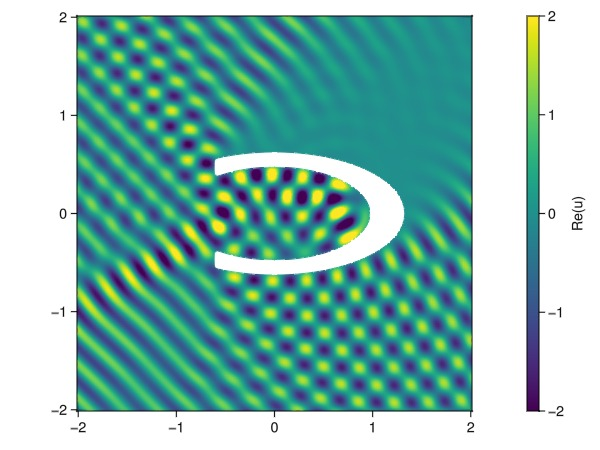
\includegraphics[width=0.5\linewidth]{images/cavity_fig.jpg}
    \caption{Geometry used in the test.}
    \label{fig:cavity_fig}
\end{figure}


We begin by running smaller examples and study the bounds found of \autoref{chap:gmres}, mainly \ref{eq:bound_E} and \ref{eq:boundE_final}. Satisfying these bounds is a guarantee that the residual measured at each k-th iteration, $\tilde{r_{k}}$, is close to the exact one $r_{k} =b-Ax_{k}$.

%FIXME: Expliquer le setup numerique: qu est ce qu'on met la et qu est ce que ça veut dire

This test run was executed with a smaller $A$, of dimensions $1650\times 1650$, and we use $\epsilon = 10^{-8}$ to assemble the hierarchical matrix as well as the algorithm's overall tolerance, i.e., the iterations stop as soon as $\frac{\norm{b - Ax_{k}}}{\norm{b}} \leq \epsilon$. The plots are in \autoref{fig:bound44}.

\begin{figure}[h!]
    \centering
    \begin{subfigure}[b]{0.5\linewidth}
        \includesvg[width=\linewidth]{images/bound_study.svg}
        %\label{fig:bound44_norm}
        \caption{Evolution for the upper bound of $||E_{k}||$, using $\ell_{k}=1$ and $\ell_{k}=\frac{\sigma_{k}(H_{k})}{k}$.}
    \end{subfigure}

    \begin{subfigure}[b]{0.3\linewidth}
        \includesvg[width=\linewidth]{images/bounds_44_normal.svg}
        %\label{fig:bound44_norm}
        \caption{Evolution of the upper bound in $\norm{r_{k} - \tilde{r_{k}}}$ for the case $\ell_{k}=1$.}
    \end{subfigure}
    \begin{subfigure}[b]{0.3\linewidth}
        \includesvg[width=\linewidth]{images/bounds_44_sing.svg}
        %\label{fig:bound44_sing}
        \caption{Evolution of the upper bound in $\norm{r_{k} - \tilde{r_{k}}}$ for the case $\ell_{k}=\frac{\sigma_{k}(H_{k})}{k}$.}
    \end{subfigure}
    \caption{Upper bound study for the perturbation and residuals involved in the cavity scattering problem. The hierarchical matrix was assembled with a $10^{-8}$ tolerance.}
    \label{fig:bound44}
\end{figure}

The bigger picture in \autoref{fig:bound44} shows how the different bounds of the perturbation's behave through iterations. Recalling that a greater tolerance means a bigger room to work with larger perturbations of $A$, what can make the inexact matrix-vector product faster.

The plot shows choosing $\ell_{k} = 1$, what makes the inexact product's tolerance bigger, i.e., “allows” for a more perturbed $A$, still respects the restriction in the bound \ref{eq:borne_delta}, as we can see on the left smaller plot. This shows bigger tolerances can still be used to achieve higher acceleration, while still maintaining the residual in a proper value. The different heuristics for the product tolerances at each iteration did not result in big variations in the total amount of iterations for the Inexact GMRES.

Passing on to the speed-up evaluation, we repeat a similar numeral setup: $A$ is assembled using the overall tolerance $\epsilon = 10^{-8}$. All product tolerances for each iteration, $\nu_{k}$, are obtained through the heuristic in \ref{eq:gen_heuristics}. We fix $A$'s dimensions as a $40000\times 40000$ matrix, and change the overall tolerance passed to the algorithm, varying from $10^{-8}$ to $10^{-2}$. The speed-up results for this fixed size test, as well as their respective relative residuals, are in \autoref{fig:cavity_results}.

\begin{figure}[h!]
    \centering
    \begin{subfigure}[b]{0.6\linewidth}
        \includesvg[width=\linewidth]{images/cavity_fixsize_speedup.svg}
        \caption{Speed-up measured for the fixed size cavity scattering problem.}
    \end{subfigure}
    \begin{subfigure}[b]{0.4\linewidth}
        \includesvg[width=\linewidth]{images/cavity_fixsize_residual.svg}
        \caption{Relative residual measured for the fixed size cavity scattering problem.}
    \end{subfigure}
    \begin{subfigure}[b]{0.4\linewidth}
        \includesvg[width=\linewidth]{images/cavity_fixsize_iterations.svg}
        \caption{Number of iterations for the fixed size cavity scattering problem.}
    \end{subfigure}
    \caption{Speed-up, relative residual and amount of iterations results for the Inexact GMRES algorithm in the cavity scattering problem. The hierarchical matrix $A$ was assembled with $10^{-8}$ tolerance and had a fixed $40000 \times 40000$ size.}
    \label{fig:cavity_results}
\end{figure}

As we can see, the speed-up did not cause a worse relative residual for the solution, always keeping it under the overall tolerance $\epsilon$ given for the algorithm. But, we can see the existence of a trade-off between tolerance and speed-up: lower precision in the algorithm may lead to a slower execution. The different number of iterations needed for each run, also in \autoref{fig:cavity_results}, shows that the slower results in the lower tolerance rate are not result of a larger number iterations, but maybe heavier ones in comparison to the exact algorithm.

For the last numerical setup, we again assemble $A$ with $10^{-8}$ tolerance, but now its dimensions will change while keeping the overall tolerance passed to the algorithm, $\epsilon$, fixed at $10^{-4}$.

\begin{figure}[h!]
    \centering
    \begin{subfigure}[b]{0.6\linewidth}
        \includesvg[width=\linewidth]{images/cavity_fixtol_speedup.svg}
        \caption{Speed-up measured for the fixed tolerance cavity scattering problem.}
    \end{subfigure}
    \begin{subfigure}[b]{0.4\linewidth}
        \includesvg[width=\linewidth]{images/cavity_fixtol_residual.svg}
        \caption{Relative residual for the fixed tolerance cavity scattering problem.}
    \end{subfigure}
    \begin{subfigure}[b]{0.4\linewidth}
        \includesvg[width=\linewidth]{images/cavity_fixtol_iterations.svg}
        \caption{Number of iterations for the fixed tolerance cavity scattering problem.}
    \end{subfigure}
    \caption{Speed-up, relative residual and amount of iterations results for the Inexact GMRES algorithm in the cavity scattering problem. The hierarchical matrix $A$ was assembled with $10^{-8}$ tolerance and used a overall tolerance $\epsilon = 10^{-4}$ to the algorithm.}
    \label{fig:cavity_resultsfixtol}
\end{figure}
